\documentclass{article}
\usepackage{../lambdatex} %disponibile all'indirizzo http://lambdamath.altervista.it/esercizi/lambdatex.sty
\usepackage{tasks}
\usepackage{exsheets}
\newcommand{\se}{\text{ se }}
\renewcommand{\phi}{\varphi}
\everymath{\displaystyle}

\title{Università degli Studi di Trento - Dipartimento di Matematica\\
CdL in Matematica – a.a. 2022–2023\\ Note esercitazione}
\author{Esercitatore: Simone Verzellesi\thanks{Trascrizione a cura di Davide Borra}}
\date{07 Dicembre 2022}
\begin{document}
\maketitle
\lhead{Note esercitazione}
\chead{Università degli Studi di Trento - Dipartimento di Matematica\\
CdL in Matematica – a.a. 2022–2023}
\rhead{07/12/2022}
\setlength{\headheight}{30pt}
% \begin{question}
%     pippo
%\end{question}
\begin{enumerate}[label=\textbf{Esercizio 11.\arabic*.},itemindent=*]
%%%%%%%%%%%%%%%%%%%%%%%%%%%%%%%%%%%%%%%%%%%%%%%%%%%%%
\item Siano $\beta\in \R$ e $S_\beta$ l'area del sottografico associato alla funzione $f(x)=x^2+\beta$ dove $x\in [-2,2]$.
\begin{tasks}
    \item disegnare la regione di piano $S_\beta$
    \item calcolare $S_\beta$
\end{tasks}
\item[\textit{\large Soluzione~}]~
Dobbiamo distinguere tre casi:
\begin{figure}[h]
    \centering
    \begin{subfigure}{0.27\textwidth}
        \centering
        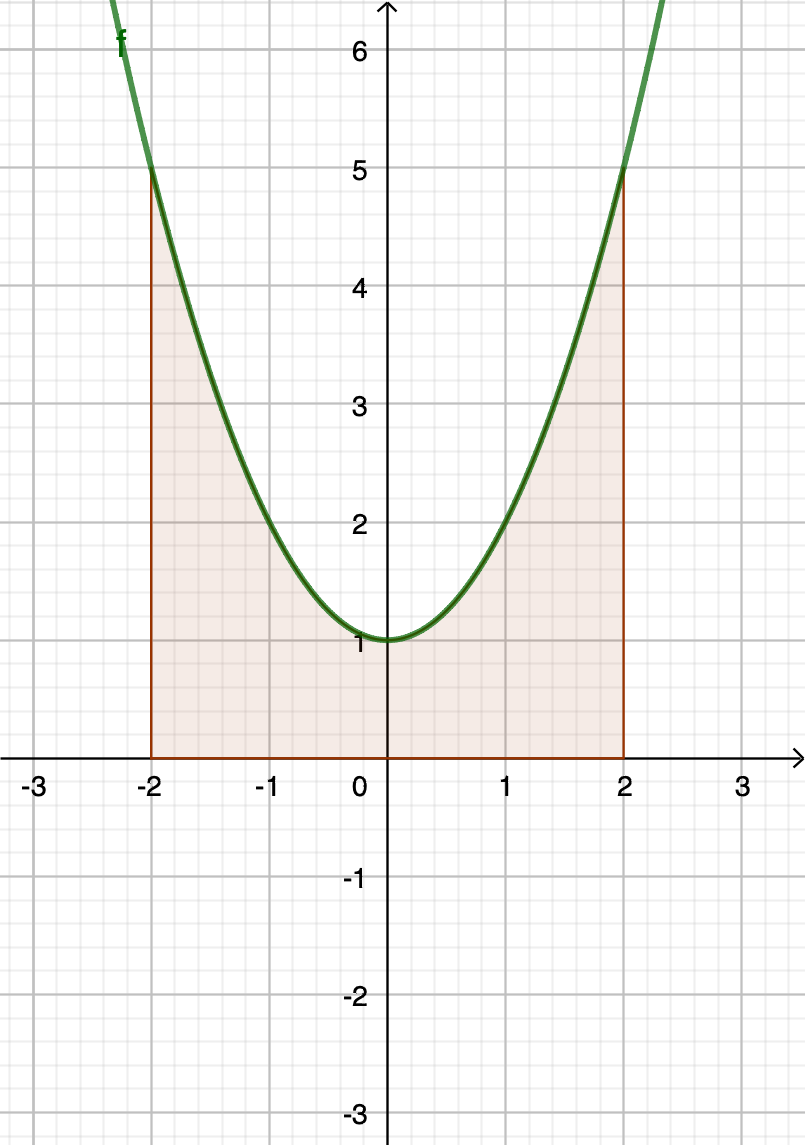
\includegraphics[width=.9\textwidth]{src/caso1.png}
        \caption{$\beta>0$}
        \label{subfig:caso1}
    \end{subfigure}
    \begin{subfigure}{0.27\textwidth}
        \centering
        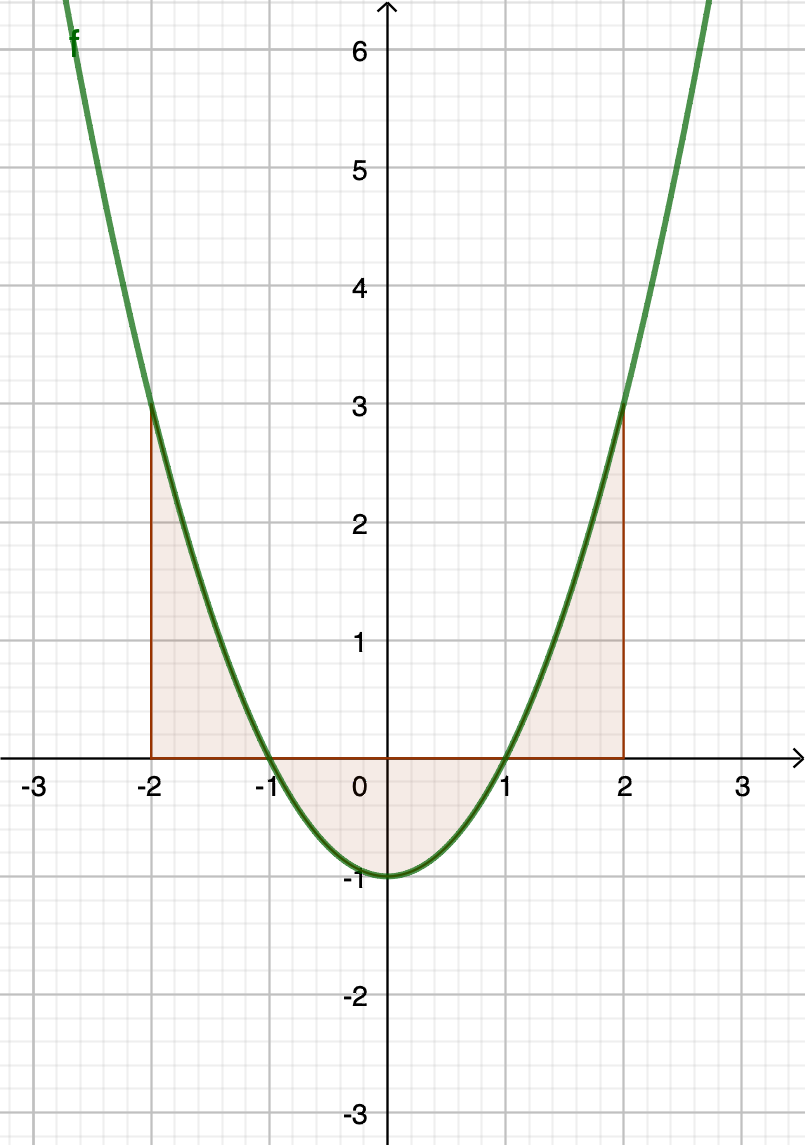
\includegraphics[width=0.9\textwidth]{src/caso2.png}
        \caption{$-4\leq\beta<0$}
        \label{fig:caso2}
    \end{subfigure}
    \begin{subfigure}{0.27\textwidth}
        \centering
        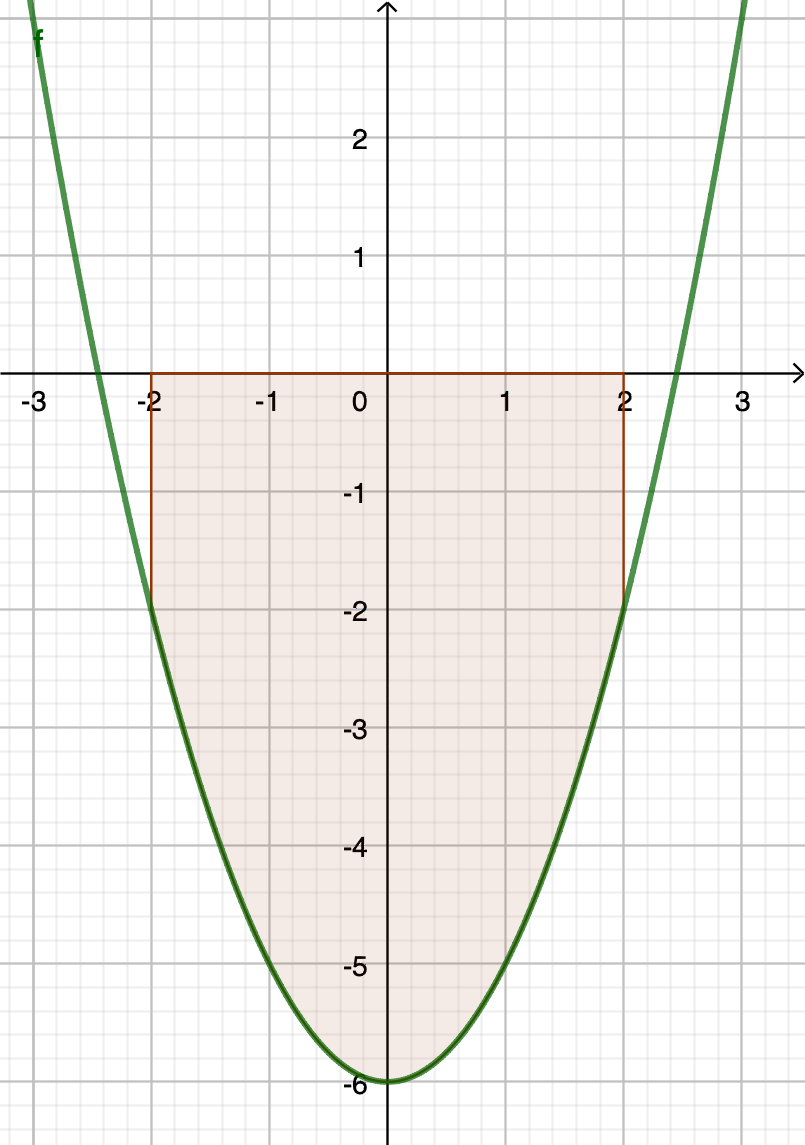
\includegraphics[width=.9\textwidth]{src/caso3.png}
        \caption{$\beta<-4$}
        \label{fig:caso3}
    \end{subfigure}
    \caption{}
\end{figure}
\begin{itemize}
    \item $\beta\geq0$ In questo caso la parabola si trova sempre sopra l'asse $x$ (Figura \ref{subfig:caso1}). \[S_\beta=\int_{-2}^2(x^2+\beta)dx.\]
    \item Analizziamo ora quando la parabola interseca l'asse $x$ in due punti interni all'intervallo $[-2,2]$ (Figura \ref{fig:caso2})
    \[x^2+\beta=0~~\Harr~~x^2=-\beta~~\Harr~~x=\pm\sqrt{-\beta}\]
    \[\implies \exists x \in [-2,2]~:~f(x)=0~~\Harr -\beta\leq 4~~\Harr~~\beta\geq -4\]
    Di conseguenza, quando $-4\leq \beta<0$
    \[S_\beta=\int_{-2}^{2}|f(x)|dx=\int_{-2}^{-\sqrt{-\beta}}(x^2+\beta)dx -\int_{-\sqrt{-\beta}}^{\sqrt{-\beta}}(x^2+\beta)dx+\int_{\sqrt{-\beta}}^{2}(x^2+\beta)dx.\]
    \item Rimane il caso in cui la parabola si trova sempre sotto l'asse $x$ in $[-2,2]$, ovvero quando $\beta<4$ (Figura \ref{fig:caso3}), in cui si ha
    \[S_\beta=-\int_{-2}^2(x^2+\beta)dx.\]
\end{itemize}

%%%%%%%%%%%%%%%%%%%%%%%%%%%%%%%%%%%%%%%%%%%%%%%%%%%%%
\item Determinare l'area della regione di piano compresa tra $f(x)=\cos x$ e $g(x)=\sin x$ e le rette $x=0$ e $x=\pi$.
\item[\textit{\large Soluzione~}]~
Prima di tutto determiniamo l'intersezione di $f$ e $g$ su $\left[ 0,\pi \right]$:
\[f(x)=g(x)~~\Harr~~x=\frac{\pi}{4}.\]
\begin{figure}[h]
    \centering
    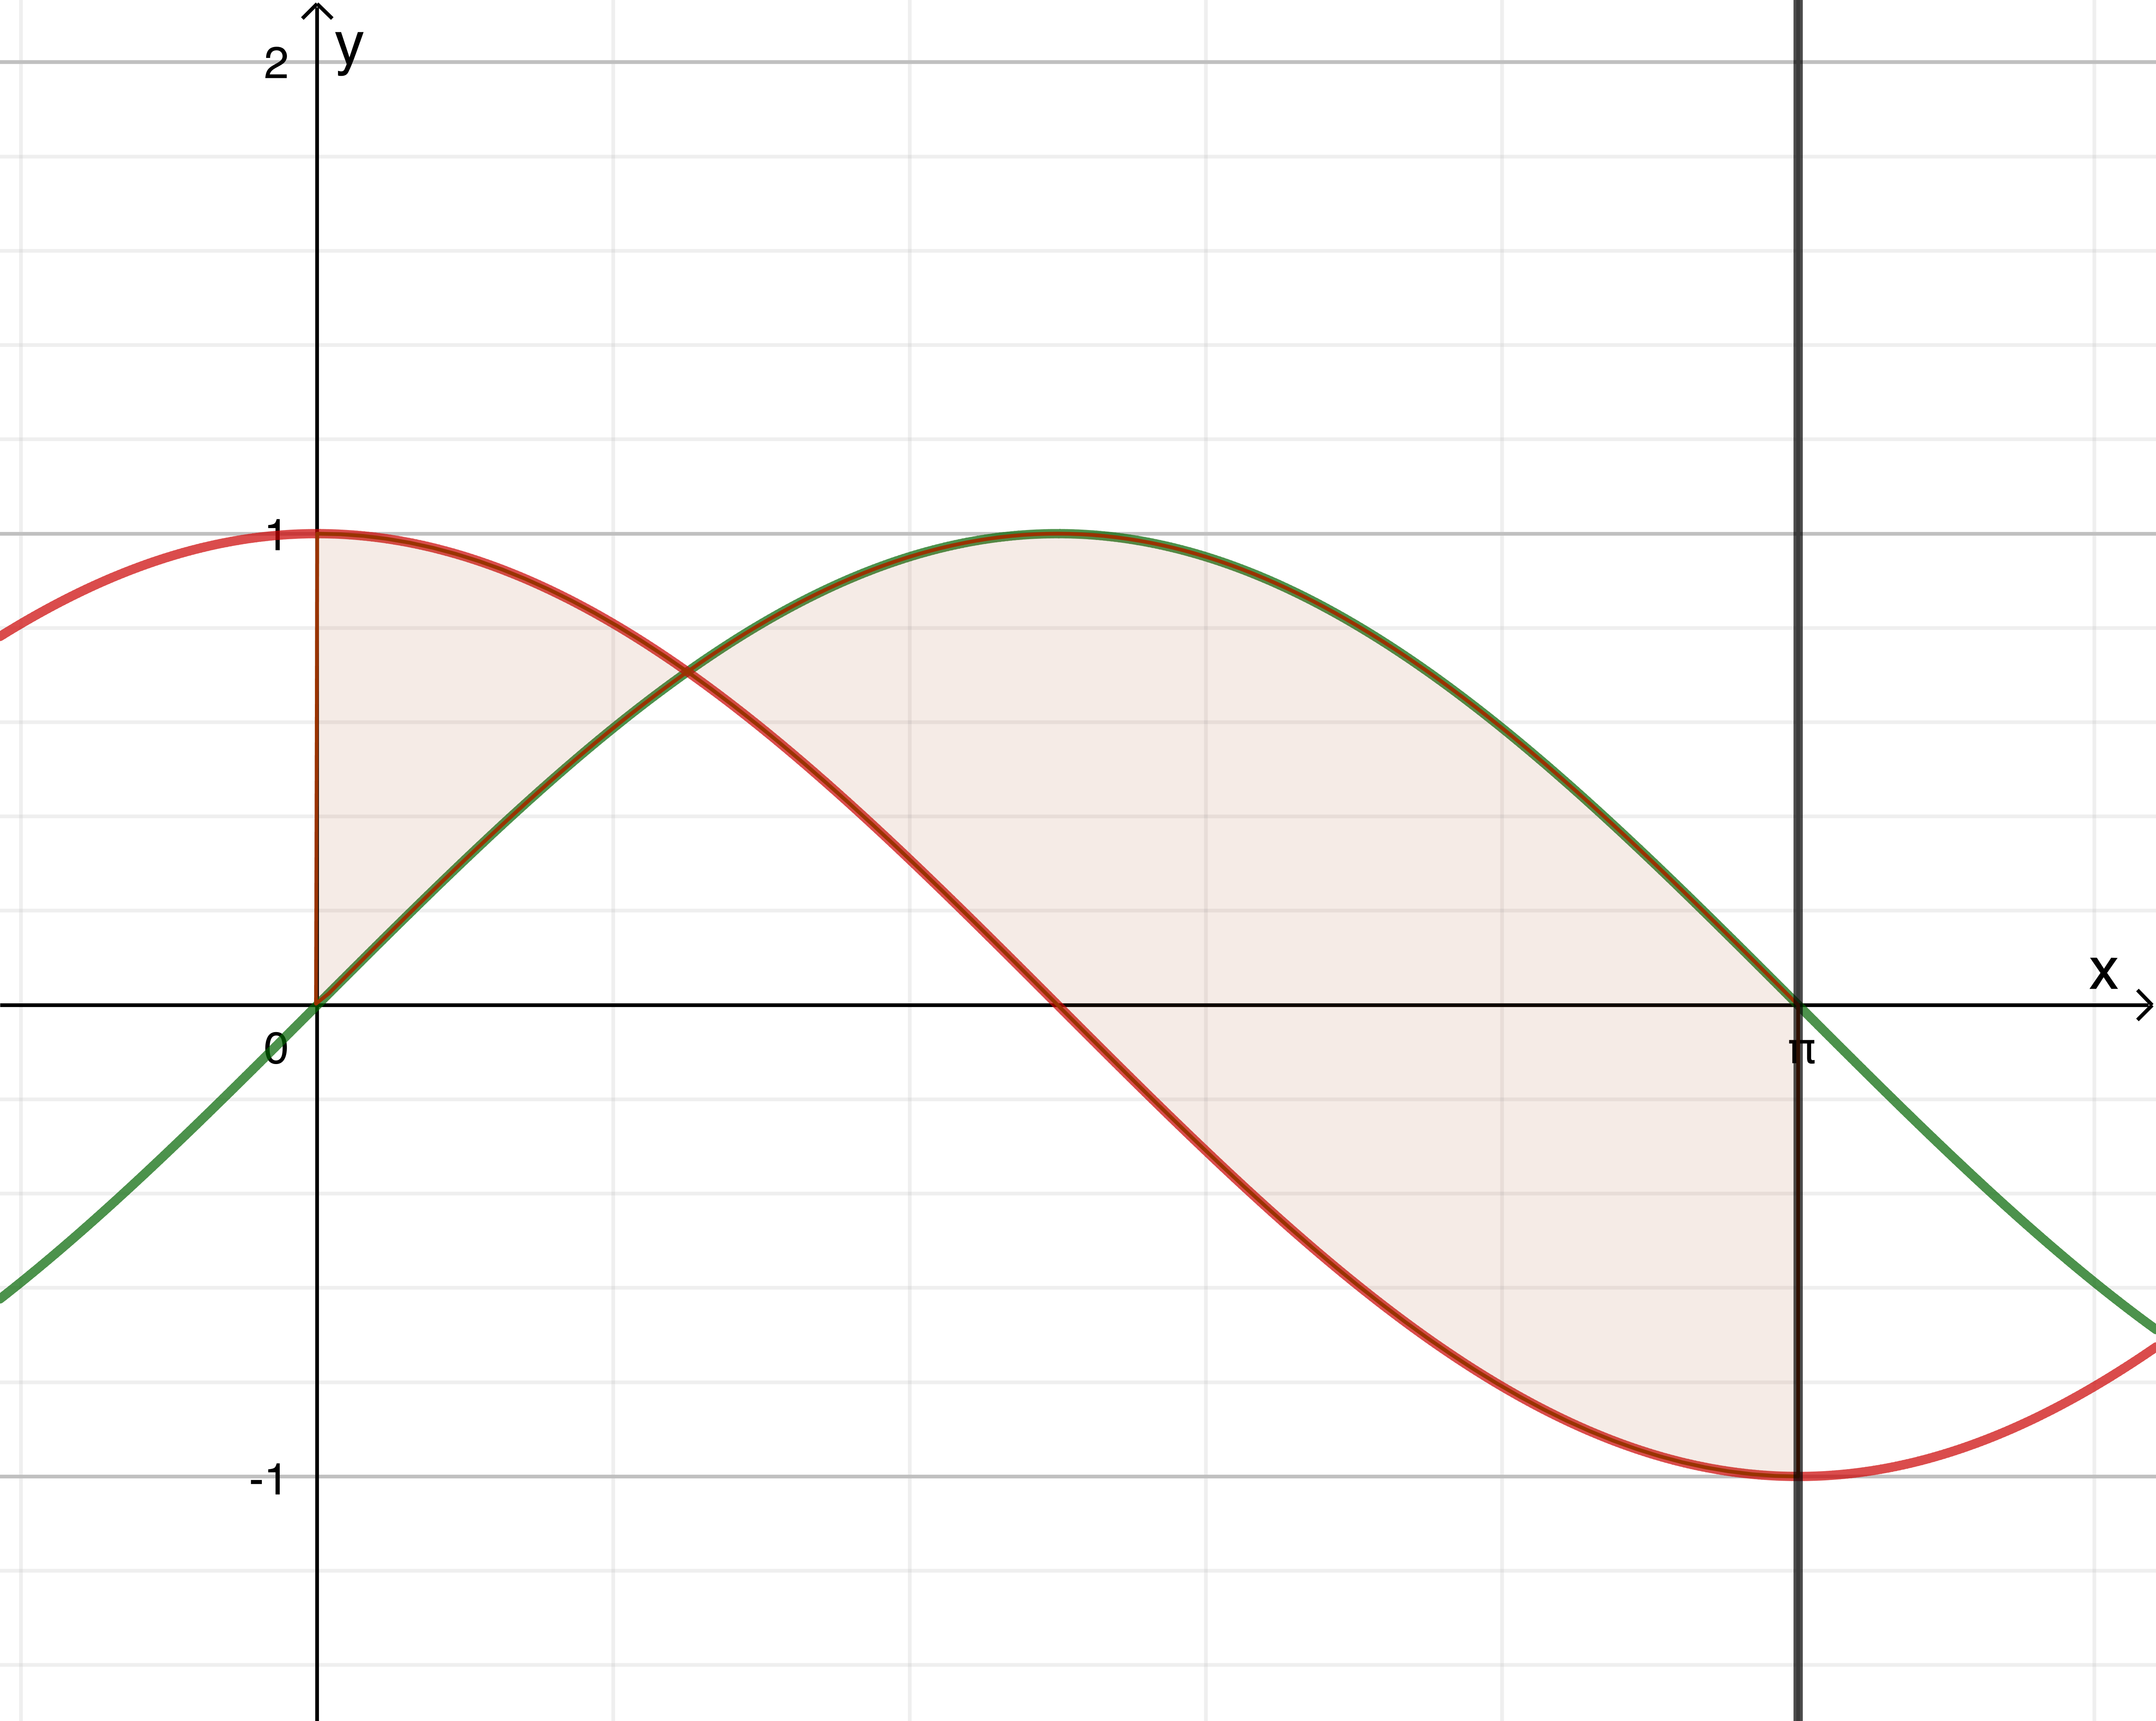
\includegraphics[width=0.5\textwidth]{src/es2.png}
    \caption{In rosso il grafico di $f$, in verde il grafico di $g$. L'intersezione si ha per $x= \frac{\pi}{4}$}
    \label{fig:es2}
\end{figure}
Abbiamo quindi che $f(x)\geq g(x)$ su $\left[ 0,\frac{\pi}{4} \right]$ e che $f(x)\leq g(x)$ su $\left[ \frac{\pi}{4} , \pi\right]$.
Di conseguenza 
\[\begin{aligned}A&=\int _0^{\frac{\pi}{4}}(\cos x-\sin x)dx-\int_{\frac{\pi}{4}}^\pi(\cos x -\sin x)dx=[\sin x+\cos x]_0^{\frac{\pi}{4}}-[\sin x+\cos x]_{\frac{\pi}{4}}^\pi=\\ &=\left(\frac{\sqrt{2}}{2}+\frac{\sqrt{2}}{2}-0-1\right)-\left(0-1 -\frac{\sqrt{2}}{2}-\frac{\sqrt{2}}{2}\right)=2\sqrt{2}.\end{aligned}\]
%%%%%%%%%%%%%%%%%%%%%%%%%%%%%%%%%%%%%%%%%%%%%%%%%%%%%
\item Calcolare i seguenti integrali definiti
\begin{tasks}(4)
    \task \(\int_{1}^{2}\frac{x+2\sqrt[3]{x}}{x^2}dx\)
    \task \(\int_{9}^{16}\frac{\sqrt{x}-3}{x-3\sqrt{x}+2}dx\)
    \task \(\int_{0}^{e-\frac{1}{e}}\sqrt{4 +x^2}dx\)
    \task \(\int\frac{1}{1+\sin x}dx.\)
\end{tasks}
\item[\textit{\large Soluzione~}]~
\begin{tasks}
    \task \(\int_{1}^{2}\frac{x+2\sqrt[3]{x}}{x^2}dx=\int_1^2\frac{1}{x}dx+2\int_1^2x^{-\frac{5}{3}}dx=\left[\log x-3x^{-\frac{2}{3}}\right]_1^2=\log2-3\cdot 2^{-\frac{2}{3}}+3.\)
    \task \(\int_{9}^{16}\frac{\sqrt{x}-3}{x-3\sqrt{x}+2}dx\)\\
    Risolviamo per sostituzione: sia $t=\sqrt{x}~~\Rarr~~x=t^2~~\Rarr dx=2tdt$. Modifichiamo di conseguenza gli estremi di integrazione: $x_0 =9~~\Rarr~~t_0=3$ e $x_1 =16~~\Rarr ~~t_1=4$
    \[\int_{9}^{16}\frac{\sqrt{x}-3}{x-3\sqrt{x}+2}dx=\int_3^4\frac{t-3}{t^2-3t+2}2tdt=2\int _3^4\frac{t^2-3t+2-2}{t^2-3t+2}dt=2\int_3^4dt-4\int_3^4 \frac{1}{t^2-3t+2}dt\]
    Adesso scomponiamo la frazione con il metodo dei fratti semplici
    \[\frac{1}{t^2-3t+2}=\frac{1}{(t-2)(t-1)}=\frac{A}{t-2}+\frac{B}{t-1}=\frac{A(t-1)+B(t-2)}{(t-2)(t-1)}=\frac{(A+B)t-(A+2B)}{(t-2)(t-1)},\]
    da cui \[\begin{cases}
        A+B=0\\A+ 2B=-1
    \end{cases}~~\Harr~~\begin{cases}
        A=-B=1\\B=-1
    \end{cases}.\]
    Quindi
    \[2\int_3^4dt-4\int_3^4 \frac{1}{t^2-3t+2}dt=2- 4\left( \int_3^4\frac{1}{t-2}dt -\int_3^4\frac{1}{t-1}dt\right)=2-4\left[ \log|t-2| -\log|t-1|\right]_3^4=\]\[=2-4\log2+4\log3-4\log2=2+4\log\frac{3}{4}.\]
    \task \(\int_{0}^{e-\frac{1}{e}}\sqrt{4 +x^2}dx\)\\
    Quando si presentano situazioni del genere è utile sostituire applicando le relazioni tra seno e coseno o tra seno e coseno iperbolici. In particolare se si presenta $\sqrt{1-x^2}$ è utile sostituire ricordando che $\cos^2x+\sen^2x=1$, mentre se si presenta $\sqrt{1+x^2}$ è utile sostituire ricordando che $\cosh^2x-\senh^2x=1$. In questo caso sostituiamo $x=2\sinh t$, quindi $dx=2\cosh t dt$. Di conseguenza gli estremi di integrazione diventano $t_0=0$ e $t_1=1$.
    \[
    \begin{aligned}
        \int_{0}^{e-\frac{1}{e}}\sqrt{4 +x^2}dx&= 4\int_0^1\sqrt{4+4\senh^2t}\cdot 2\cosh tdt=4\int_0^1\sqrt{\cosh^2t}\cosh t dt= 4\int_0^1\cosh^2 tdt=\\&=4\int_0^1\cosh t\cosh t dt=4\left( \biggl[ \sinh t\cosh t \biggr]_0^1-\int_0^1\senh^2tdt \right)=\\&=4\int_0^1\cosh t\cosh t dt=4\left( \biggl[ \sinh t\cosh t \biggr]_0^1-\int_0^1(\cosh^2t-1)dt \right)=\\&=4\left( \biggl[\senh t\cosh t\biggr]_0^1+\int _0^1dt-\int_0^1\cosh^2tdt \right).
    \end{aligned}\]
   Risulta quindi 
    \[8\int_0^1\cosh^2tdt=4\biggl[\senh t\cosh t +t\biggr]_0^1.\]
   Concludiamo
    \[\begin{aligned}\int_{0}^{e +\frac{1}{e}}\sqrt{4 +x^2}\d x &= 4\int_0^1\cosh^2t\d t = 2\biggl[\senh t\cosh t +t\biggr]_0^1=2\left( \frac{e-\frac{1}{e}}{2} \cdot \frac{
    e+\frac{1}{e}}{2} +1\right)= \\&=\frac{e^2 - e^{ - 2}}{2} + 2 = \sinh 2 + 2.\end{aligned}\]
    \task \(\int\frac{1}{1+\sin x}dx\)\\
    Per risolvere questo tipo di integrale bisogna utilizzare le formule parametriche di seno e coseno: sia $t=\tg\frac{x}{2}$, allora si ha $\sin x= \frac{2t}{1+t^2}$ e $\cos x= \frac{1-t^2}{1+t^2}$. Inoltre $x=2\arctg t$ e $dx =\frac{2}{1+t^2}dt$. 
    Infatti
    \[\frac{2t}{1+t^2}=\frac{2\tg\frac{x}{2}}{1+\tg^2\frac{x}{2}}=\frac{2\frac{\sin \frac{x}{2}}{\cos \frac{x}{2}}}{1+\frac{\sin ^2\frac{x}{2}}{\cos^2 \frac{x}{2}}}=\frac{2\sin \frac{x}{2}\cos \frac{x}{2}}{\cos^2\frac{x}{2}+\sin^2 \frac{x}{2}}=\sin x.\]
    Di conseguenza
    \[\begin{aligned}\int\frac{1}{1+\sin x}dx&\underset{t = \tg \frac{x}{2}}{=}\int\frac{1}{\frac{2t}{1+t^2}+1}\cdot \frac{2}{1+t^2}dt=\int \frac{2\cancel{(1+t^2)}}{(2t+1+t^2)\cancel{(1+t^2)}}dt=\\&=\int \frac{2}{(1+ t)^2}dt=-\frac{2}{1+ t}+c\bigg|_{t =\tg\frac{x}{2}}=-\frac{2}{1+\tg \frac{x}{2}}+ c.\end{aligned}\]
\end{tasks}
%%%%%%%%%%%%%%%%%%%%%%%%%%%%%%%%%%%%%%%%%%%%%%%%%%%%%
\item Studiare la convergenza di $\int_0^1\frac{\sin x}{\sqrt{x}\sqrt[4]{1-x}}dx$.
\item[\textit{\large Soluzione~}]~ Chiamiamo $f(x)$ la funzione integranda. Osserviamo che $f\in \mathcal{C}^0(]0,1[)$ e positiva. Inoltre osserviamo che per $x\to 0^+$, $\sin x\sim x$ e $\sqrt[4]{1-x}\sim 1$, quindi $f(x)\sim \frac{x}{\sqrt{x}}=\sqrt{x}$. È perciò possibile estendere con continuità la funzione $f$ in 0 con $\tilde{f}(0)=0$, per cui $f\in \mathcal{R}\left(\left[0,\frac{1}{2}\right]\right)$. Per $x\to1^-$ osserviamo che $f(x)\sim\frac{\sin 1}{\sqrt[4]{1-x}}=\frac{\sin 1}{(1-x)^{\frac{1}{4}}}$. Poiché $\int_{\frac{1}{2}}^1\frac{1}{(1-x)^{\frac{1}{4}}}\d x$ converge, allora per il teorema del confronto asintotico, anche $\int_{\frac{1}{2}}^1f(x)\d x$ converge. Di conseguenza $\int_0^1\frac{\sin x}{\sqrt{x}\sqrt[4]{1-x}}\d x$ converge.
%%%%%%%%%%%%%%%%%%%%%%%%%%%%%%%%%%%%%%%%%%%%%%%%%%%%%
\item Determinare per quali $\alpha, \beta\in \R$ l'integrale
\[\int_0^{+\infty}\frac{1}{x^\alpha(4+9x)^{\beta+1}}dx\]
converge e calcolarne il valore con $\alpha=\frac{1}{2}$ e $\beta=0$. 
\item[\textit{\large Soluzione~}]~ Chiamiamo $f(x)$ la funzione integranda. Abbiamo $f\in \mathcal{C}^0\left( \left] 0,+\infty \right[ \right)$ e positiva.
\\ Per $x\to 0^+$ si ha $f(x)\sim \frac{1}{x^\alpha}$, quindi per il teorema del confronto asintotico l'integrale dato converge se e solo se $\alpha <1$. 
\\ Per $x\to +\infty$ $f(x)\sim\frac{1}{x^\alpha(9x)^{\beta+1}}=\frac{1}{9^{\beta+1}x^{\alpha+\beta+1}}$. Affinché l'integrale converga su $[1,+\infty[$ deve essere $\alpha+\beta+1>1$, ovvero $-\beta<\alpha$.

Di conseguenza l'integrale dato converge se e solo se $-\beta<\alpha<1$.


Calcoliamo ora il valore dell'integrale nel caso $\alpha=\frac{1}{2}$ e $\beta=0$:
\[\begin{aligned}\int_0^{+\infty}\frac{1}{\sqrt{x}(4+9x)}dx&=\int_0^1\frac{1}{\sqrt{x}(4+9x)}dx+\int_1^{+\infty}\frac{1}{\sqrt{x}(4+9x)}dx=\\&=\lim_{\delta\to {0^+}}\int_\delta^1\frac{1}{\sqrt{x}(4+9x)}dx+\lim_{h\to {+\infty}}\int_1^{h}\frac{1}{\sqrt{x}(4+9x)}dx.\end{aligned}\]
Per procedere al calcolo ci serve una primitiva di $f$. Sostituiamo ponendo $t=\sqrt{x}$, $x=t^2$, $dx=2tdt$.
\[\begin{aligned}
    \int\frac{1}{\sqrt{x}(4+9x)}dx&=\int\frac{1}{t(4+9t^2)}2tdt=2\int\frac{1}{4+9t^2}dt=\frac{1}{3}\int\frac{\frac{3}{2}}{1+\frac{9}{4}t^2}dt=\frac{1}{3}\arctg\left(\frac{3}{2}t\right)+c=\\&=\frac{1}{3}\arctg\left(\frac{3}{2}\sqrt{x}\right)+c
\end{aligned}\]
Quindi 
\[\begin{aligned}
    \int_0^{+\infty}\frac{1}{\sqrt{x}(4+9x)}dx&=
    \lim_{\delta\to {0^+}}\int_\delta^1\frac{1}{\sqrt{x}(4+9x)}dx+\lim_{h\to {+\infty}}\int_1^{h}\frac{1}{\sqrt{x}(4+9x)}dx=\\&=
    \lim_{\delta\to {0^+}}\biggl[\frac{1}{3}\arctg\left( \frac{3}{2} \sqrt{x}\right)\biggr]_\delta^1+\lim_{h\to {+\infty}}\biggl[\frac{1}{3}\arctg\left( \frac{3}{2} \sqrt{x}\right)\biggr]_1^{h}=\\&=
    \lim_{\delta\to {0^+}}\biggl[\frac{1}{3}\arctg\frac{3}{2}-\frac{1}{3}\arctg\left( \frac{3}{2} \sqrt{\delta}\right)\biggr]+\lim_{h\to {+\infty}}\biggl[\frac{1}{3}\arctg\left( \frac{3}{2} \sqrt{h}\right)-\frac{1}{3}\arctg\frac{3}{2}\biggr]=\frac{\pi}{6}.
\end{aligned}\]

%%%%%%%%%%%%%%%%%%%%%%%%%%%%%%%%%%%%%%%%%%%%%%%%%%%%%
\item Studiare la convergenza di $\int_1^2\frac{1-\cos (x-1)}{(x^2-1)^\alpha(2-x)^{3-\alpha}}dx$ al variare di $\alpha \in \R$.
\item[\textit{\large Soluzione~}]~Riscriviamo l'integrale equivalentemente e sostituiamo $x-1=t$, $t=x+1$, $dx=dt$
\[\int_1^2\frac{1-\cos (x-1)}{(x^2-1)^\alpha(2-x)^{3-\alpha}}dx=\int_1^2\frac{1-\cos (x-1)}{(x-1)^\alpha(x+1)^\alpha(2-x)^{3-\alpha}}dx=\int_0^1\frac{1-\cos t}{(t)^\alpha(t+2)^\alpha(1-t)^{3-\alpha}}dt\]
Chiamiamo $f(t)$ la funzione integranda.
\begin{itemize}
    \item Per $t\to0^+$
    \[f(t)\sim\frac{1-\cos t}{t^\alpha}\cdot\frac{1}{2^\alpha}.\]
    Sviluppiamo il coseno
    \[\frac{1-\cos t}{t^\alpha}=\frac{\frac{t^2}{2}+o(t^2)}{t^{\alpha}}\sim \frac{1}{2t^{\alpha - 2}}.\]
    L'integrale converge se e solo se $\alpha-2<1~~\Harr~~\alpha<3$.
    \item Per $t\to1^-$ osserviamo che $1-\cos t$, $t^\alpha$ e $(t+2)^\alpha$ non influiscono se non per costanti, quindi a meno di costanti
    \[f(t)\sim \frac{1}{(1-t)^{3-\alpha}}\]
    e l'integrale $\int_{\frac{1}{2}}^1f(t)dt$ converge se e solo se $3-\alpha <1~~\Harr~~\alpha>2$.
\end{itemize}
Di conseguenza l'integrale converge se e solo se 
\[2<\alpha<3.\]
%%%%%%%%%%%%%%%%%%%%%%%%%%%%%%%%%%%%%%%%%%%%%%%%%%%%%


\end{enumerate}
\end{document}
